On comparing $\myvec{1 & -2}\vec{x} = 3$ with Formulae 1  we get 
\begin{align}
\vec{n}_1^T=\myvec{1 & -2}
\end{align}
Let the normal vector of the other line is
\begin{align}
\vec{n}_2=\myvec{-m\\1}  
\end{align}
Angle between these two lines is 45\degree
\begin{align}
    \theta=45\degree
    \implies \cos 45\degree &=\frac{1}{\sqrt{2}}\\ 
\end{align}
Substituting $\vec{n}_1^T \vec{n}_2$ and $\cos\theta$ in Formulae 2  we get
\begin{align}
    \frac{1}{\sqrt{2}}=\frac{\myvec{1 & -2}\times\myvec{-m\\1}}{\sqrt{5}\times\sqrt{m^2+1}}
\end{align}
\begin{align}
    3m^2-4m-3=0
\end{align}
Solving this equation we get two roots
\begin{align}
m_1=3\\
m_2=-\frac{1}{3}
\end{align}
Equations of Line with Slope $m_1=3$ and passing through point $\myvec{3\\2}$ is given as
\begin{align}
   \vec{n}^T(\vec{x}-\vec{A})=0\\
   \vec{n}^T=\myvec{-3 & 1}
\end{align}
Substituting Values we get
\begin{align}
 \myvec{-3 & 1}\brak{\vec{x}-\myvec{3\\2}}=0\\
 \myvec{-3 & 1}\vec{x}=-7
\end{align}
Equations of Line with Slope $m_2=-\frac{1}{3}$ and passing through point $\myvec{3\\2}$ is given as
\begin{align}
\vec{n}^T(\vec{x}-\vec{A})=0\\
\vec{n}^T=\myvec{-\frac{1}{3} & 1}
\end{align}
Substituting Values we get
\begin{align}
 \myvec{\frac{1}{3} & 1}\brak{\vec{x}-\myvec{3\\2}}=0\\
 \myvec{\frac{1}{3} & 1}\vec{x}=3
\end{align}
the equation of lines through the point \myvec{3\\2}  which make an angle of 45\degree to the line
\begin{align}
\myvec{1 & -2}\vec{x} = 3 
\end{align}
are
\begin{align}
   \myvec{-3 & 1}\vec{x}=-7\\ 
   \myvec{\frac{1}{3} & 1}\vec{x}=3
\end{align}
The Figure \ref{fig:solution_line_pane_49}
shows the plot of all three lines
\begin{figure}[!ht]
\centering
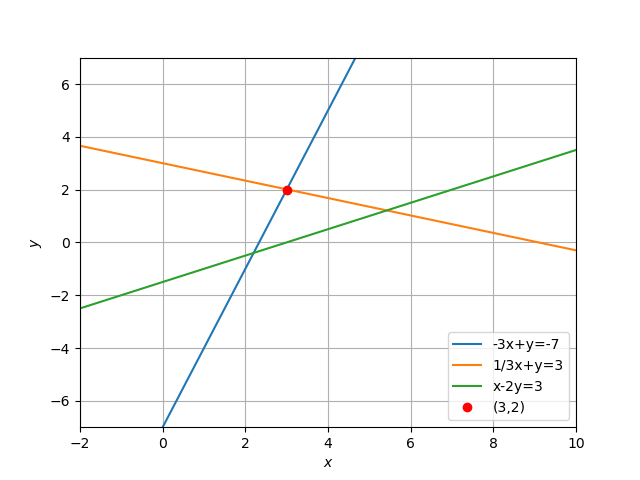
\includegraphics[width=\columnwidth]{./solutions/line_plane/49/Edit_plot.png}
\caption{Plotting these Equation}
\label{fig:solution_line_pane_49}
\end{figure}
